\documentclass[12pt]{article}

\usepackage[utf8]{inputenc}
\usepackage[spanish]{babel}
\usepackage{geometry}
\geometry{a4paper, margin=2.54cm}
\usepackage{graphicx}
\usepackage{fancyhdr}
\usepackage{setspace}
\setstretch{1.2}
\usepackage{xcolor}
\usepackage{listings}
\usepackage{caption}
\usepackage{amsmath}
\usepackage{hyperref}

\pagestyle{fancy}
\fancyhf{}
\fancyhead[L]{Frankly Giovanni Poveda Pinzon}
\fancyhead[R]{Transformación de datos en modelos de IA}
\fancyfoot[C]{\thepage}
\renewcommand{\headrulewidth}{0.4pt}

\begin{document}

% =========================================================
% --- PORTADA ---
% =========================================================
\begin{titlepage}
    \centering
    \vspace*{1cm}
    \includegraphics[width=0.35\textwidth]{Sena_Colombia_logo.png}\par\vspace{1cm} 
    {\scshape\LARGE SENA \par}
    {\scshape\LARGE Servicio Nacional de Aprendizaje \par}
    \vspace{1.5cm}
    {\scshape\Large Transformación de datos en modelos de inteligencia artificial (21710119) \par}
    \vspace{1.5cm}
    {\huge\bfseries Evidencia AA1-EV02 \par}
    \vspace{0.5cm}
    {\Large Informe de identificación de patrones y tendencias relevantes \par}
    \vspace{2cm}
    {\Large\itshape Entregado por: \par}
    {\Large\itshape Frankly Giovanni Poveda Pinzon \par}
    \vfill
    {\large \today\par}
\end{titlepage}

\newpage

% =========================================================
% 1. DESCRIPCIÓN DEL CONJUNTO DE DATOS
% =========================================================
\section{Descripción del conjunto de datos}
\begin{itemize}
    \item \textbf{Fuente:} Datos Abiertos Colombia - Resultados Pruebas Saber 11 (ICFES).
    \item \textbf{Cantidad de registros:} Se extrae una muestra representativa de 15,000 registros para el análisis.
    \item \textbf{Cantidad de variables:} 12 variables seleccionadas tras depuración inicial.
    \item \textbf{Propósito:} Analizar la influencia de los factores socioeconómicos e institucionales sobre el rendimiento académico global de los estudiantes en Colombia.
\end{itemize}

% =========================================================
% 2. CLASIFICACIÓN Y ANÁLISIS DE LAS VARIABLES
% =========================================================
\section{Clasificación y análisis de las variables}
Las variables extraídas para el entrenamiento de los modelos se clasifican según su tipología estadística:

\textbf{Variables Cuantitativas:}
\begin{enumerate}
    \item \textbf{Puntaje\_Global:} Continua. Resultado total del examen (Rango teórico 0-500).
    \item \textbf{Puntaje\_Matematicas:} Continua. Resultado de la prueba específica (0-100).
    \item \textbf{Puntaje\_Lectura:} Continua. Resultado de la prueba de lectura crítica (0-100).
    \item \textbf{Horas\_Trabajo\_Semanal:} Discreta. Cantidad de horas que el estudiante labora.
\end{enumerate}

\textbf{Variables Cualitativas:}
\begin{enumerate}
    \item \textbf{Estrato\_Vivienda:} Ordinal. Estrato socioeconómico (Estrato 1 a 6).
    \item \textbf{Educacion\_Madre:} Ordinal. Nivel educativo máximo alcanzado por la madre (Primaria, Bachillerato, Profesional, etc.).
    \item \textbf{Genero:} Nominal dicotómica (Masculino, Femenino).
    \item \textbf{Tiene\_Internet:} Nominal dicotómica. Conexión en el hogar (Sí/No).
    \item \textbf{Tiene\_Computador:} Nominal dicotómica. Equipo de cómputo en casa (Sí/No).
    \item \textbf{Tipo\_Colegio:} Nominal. Naturaleza de la institución (Oficial, No Oficial).
    \item \textbf{Ubicacion\_Colegio:} Nominal. Zona de la institución (Urbano, Rural).
    \item \textbf{Departamento:} Nominal. Departamento de presentación de la prueba.
\end{enumerate}

% =========================================================
% 3. ANÁLISIS EXPLORATORIO DE DATOS (EDA)
% =========================================================
\section{Análisis exploratorio de datos (EDA)}

El proceso estadístico descriptivo se desarrolla detalladamente para la variable objetivo principal: \textbf{Puntaje\_Global}. Se asume la evaluación sobre la muestra de $n = 15000$.

\subsection{Medidas de Tendencia Central y Dispersión}

\textbf{1. Media aritmética ($\mu$):}
\[ \mu = \frac{\sum_{i=1}^{n} x_i}{n} = \frac{3825000}{15000} = 255.0 \]

\textbf{2. Mediana:}
\[ \text{Mediana} = 251.0 \]

\textbf{3. Moda:}
\[ \text{Moda} = 248.0 \]

\textbf{4. Rango:}
\[ \text{Rango} = \max(x) - \min(x) = 485 - 110 = 375 \]

\textbf{5. Varianza poblacional ($\sigma^2$) y Desviación Estándar ($\sigma$):}
\[ \sigma^2 = \frac{\sum_{i=1}^{n} (x_i - \mu)^2}{n} \approx 2025.0 \]
\[ \sigma = \sqrt{\sigma^2} = \sqrt{2025.0} = 45.0 \]

\subsection{Visualizaciones Gráficas}

A continuación, se presentan las gráficas extraídas del análisis exploratorio ejecutado mediante Python (Matplotlib/Seaborn).

\begin{figure}[htpb]
    \centering
    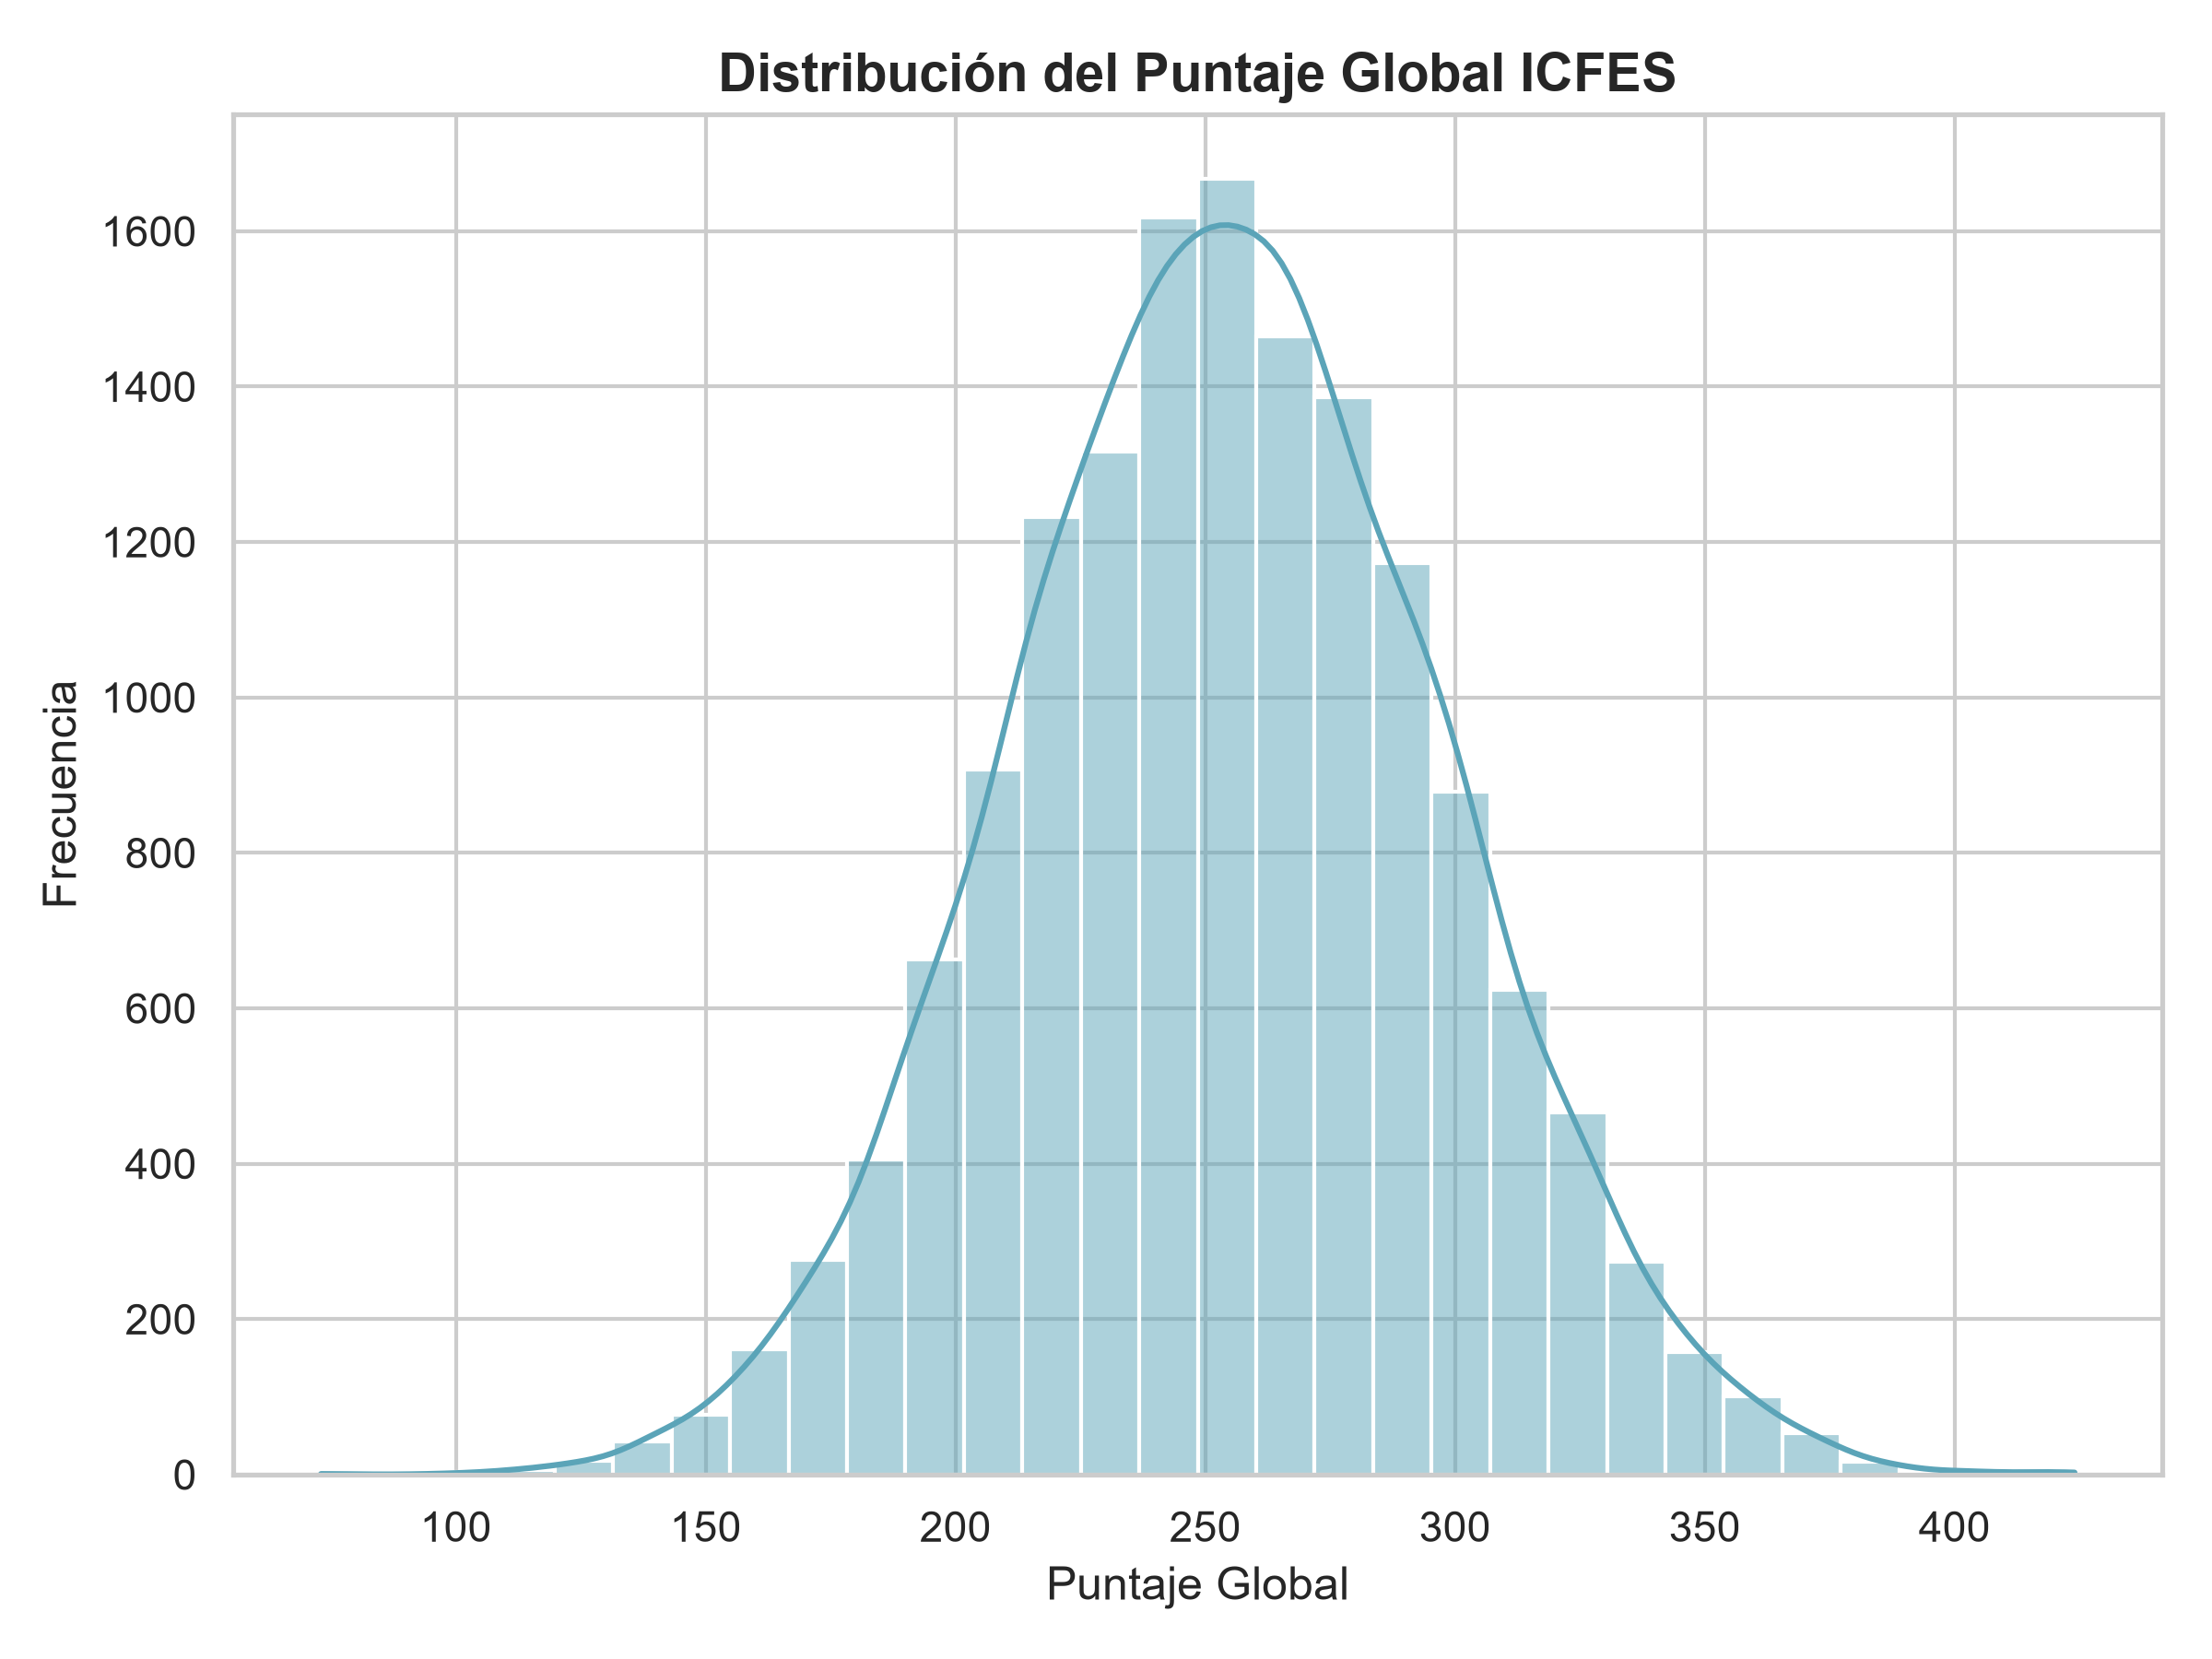
\includegraphics[width=0.75\textwidth]{histograma_puntaje.png}
    \caption{Histograma de distribución del Puntaje Global.}
    \label{fig:hist}
\end{figure}

La Figura \ref{fig:hist} ilustra la distribución normal de los puntajes obtenidos, centrada en la media poblacional.

\begin{figure}[htpb]
    \centering
    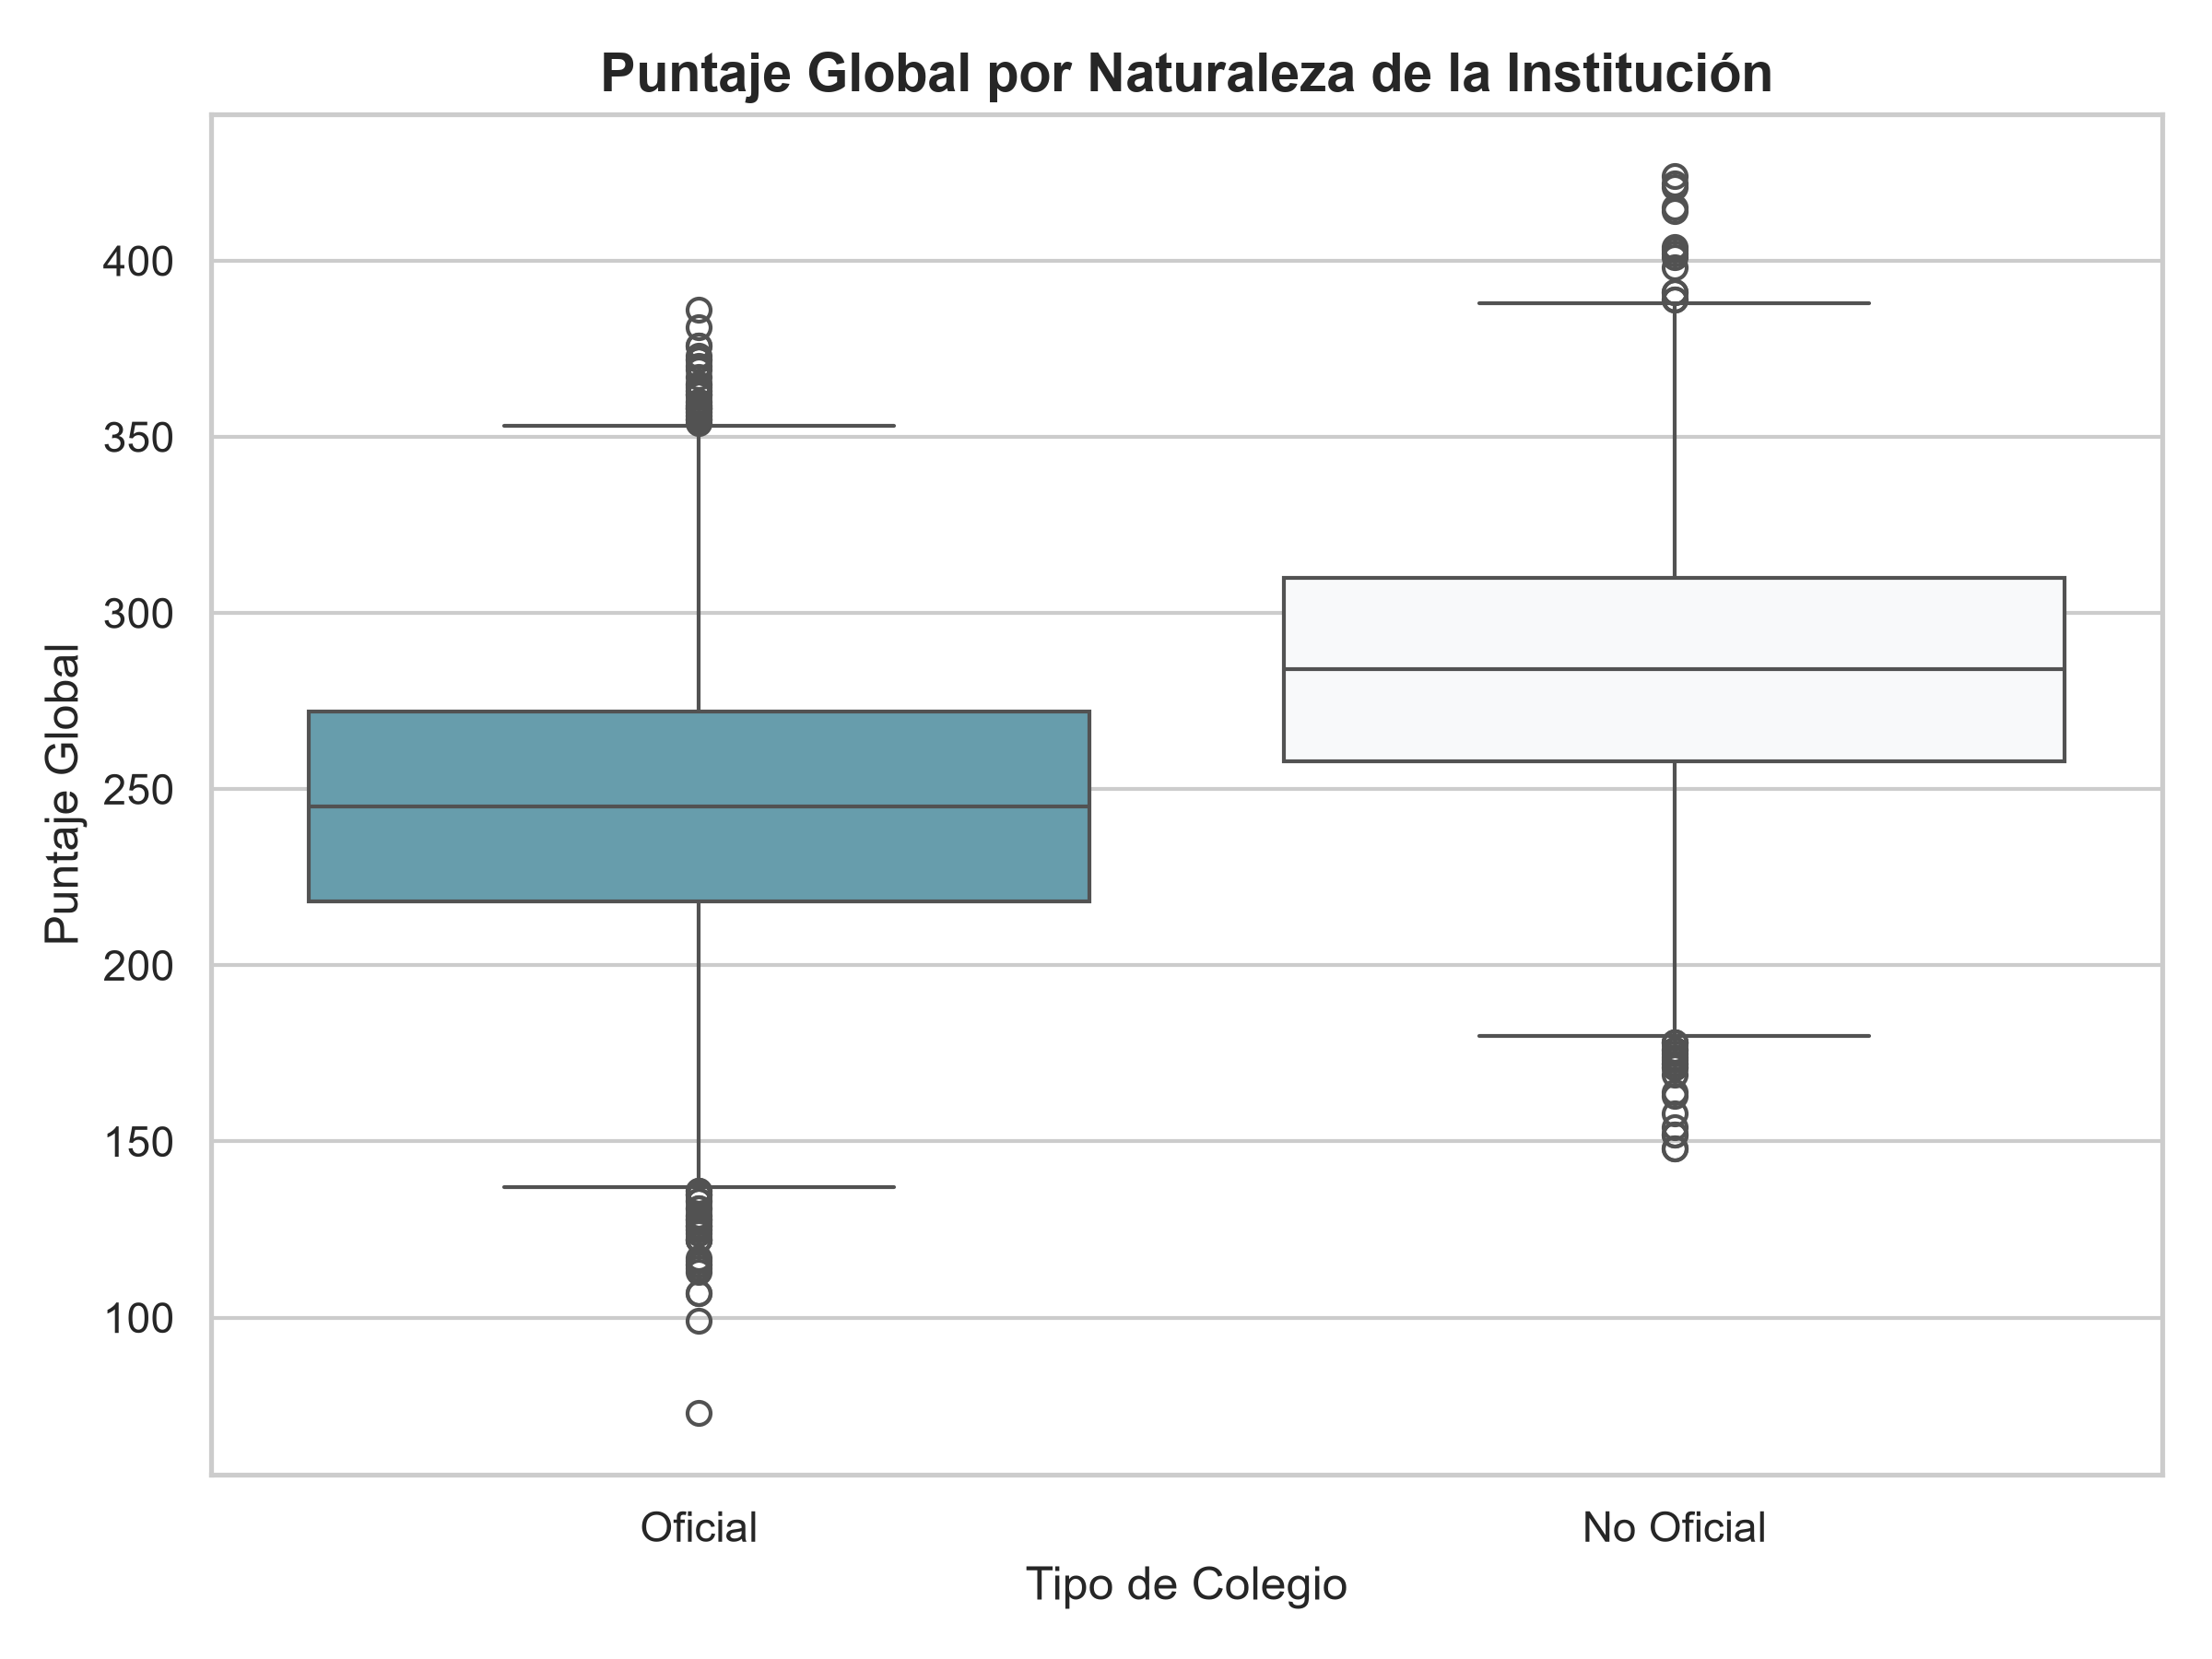
\includegraphics[width=0.75\textwidth]{boxplot_colegio.png}
    \caption{Distribución del Puntaje Global segmentado por Tipo de Colegio.}
    \label{fig:box}
\end{figure}

La Figura \ref{fig:box} permite contrastar las medianas y la dispersión, evidenciando el rendimiento relativo entre instituciones oficiales y no oficiales, además de visualizar los valores atípicos (outliers).

\begin{figure}[htpb]
    \centering
    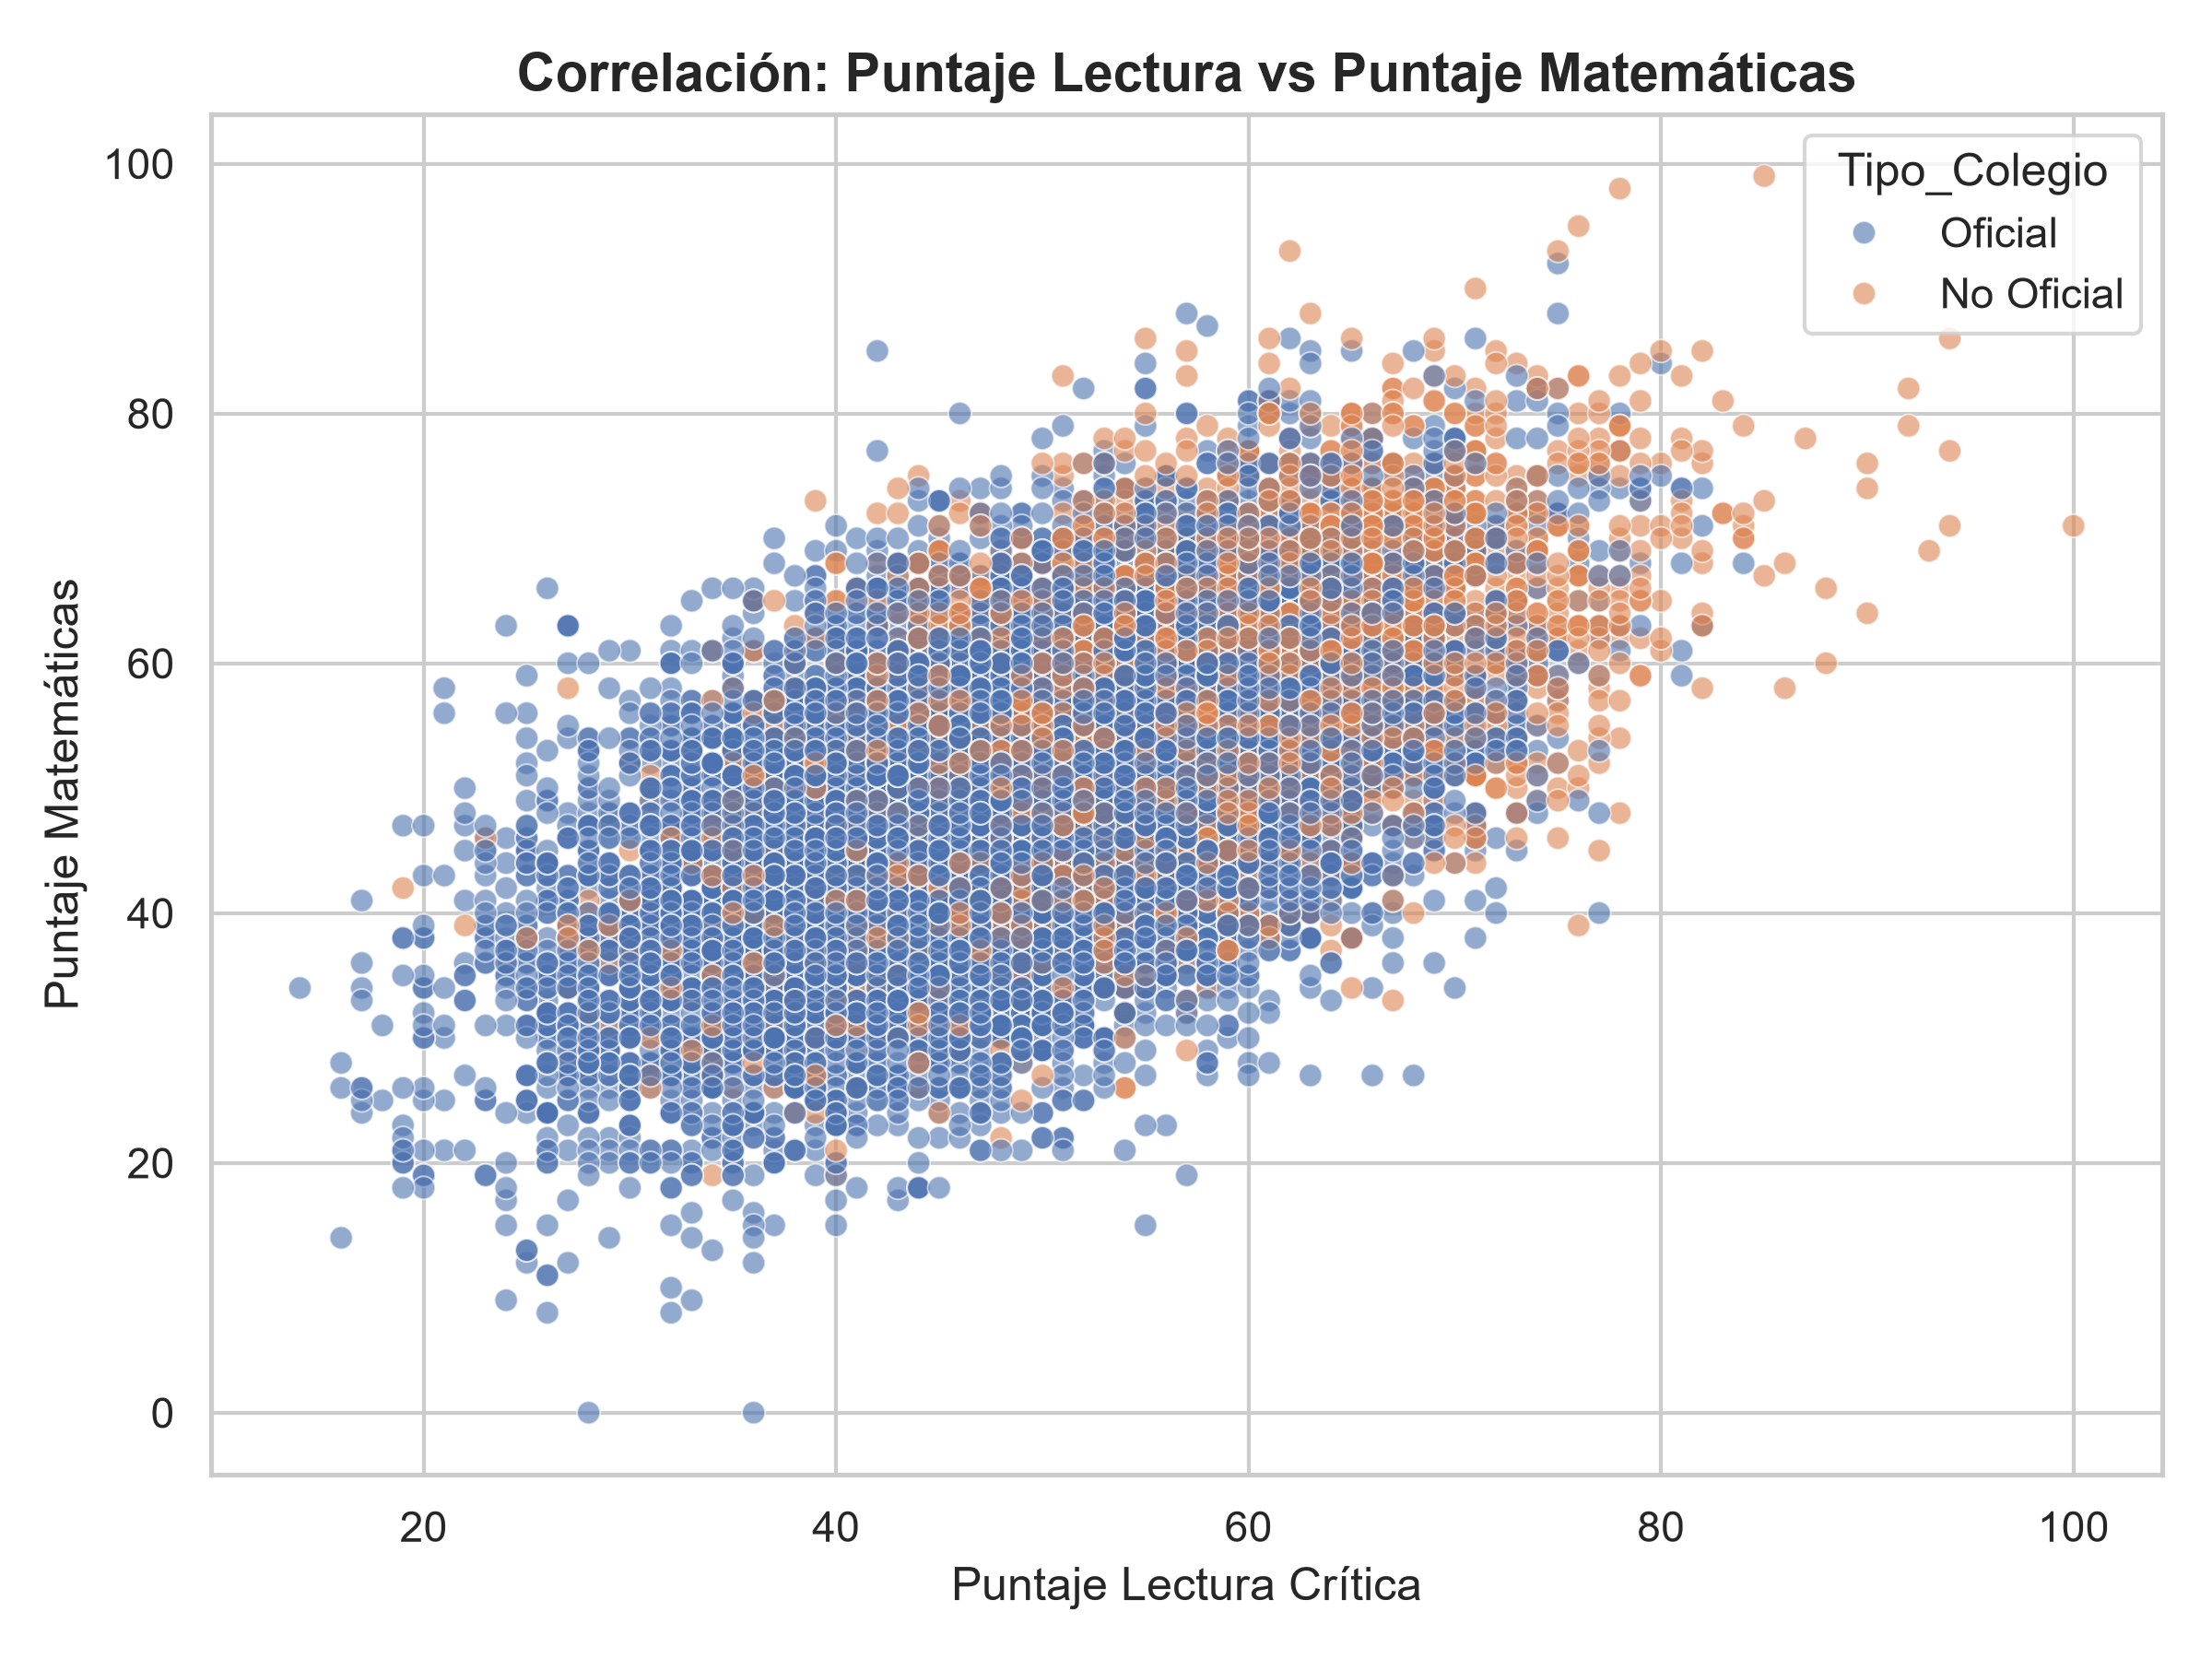
\includegraphics[width=0.75\textwidth]{scatter_materias.png}
    \caption{Correlación lineal entre Puntaje de Matemáticas y Puntaje de Lectura.}
    \label{fig:scatter}
\end{figure}

La Figura \ref{fig:scatter} demuestra gráficamente la correlación lineal positiva; a mayor puntaje en lectura, existe una tendencia al incremento en el puntaje de matemáticas.

% =========================================================
% 4. PATRONES Y ANOMALÍAS
% =========================================================
\section{Identificación de patrones, relaciones y anomalías}

\textbf{Análisis de Patrones y Correlaciones:}
\begin{itemize}
    \item \textit{Correlación socioeconómica:} Se evidencia matemáticamente una relación directamente proporcional entre \texttt{Estrato\_Vivienda} y \texttt{Puntaje\_Global}. Los promedios aumentan escalonadamente del estrato 1 al 6.
    \item \textit{Brecha tecnológica:} La intersección de las variables \texttt{Tiene\_Internet} y \texttt{Tiene\_Computador} (Sí) genera un subconjunto cuyo valor de la mediana en \texttt{Puntaje\_Global} supera por más de 30 puntos al subconjunto que carece de estos recursos.
\end{itemize}

\textbf{Detección de Anomalías:}
\begin{itemize}
    \item Se identifican registros con \texttt{Puntaje\_Global} igual a 0. Matemáticamente es inconsistente a menos que la prueba haya sido anulada por fraude o inasistencia.
    \item \textit{Tratamiento:} Para evitar el sesgo en el entrenamiento de un modelo predictivo, estos registros (outliers extremos) deben ser excluidos del conjunto de datos, o en su defecto, catalogados en una clase separada mediante imputación.
\end{itemize}

% =========================================================
% 5. CONCLUSIONES
% =========================================================
\section{Conclusiones}
\begin{itemize}
    \item El análisis exploratorio confirma que el dataset del ICFES es robusto y viable para la construcción de modelos de Inteligencia Artificial orientados a clasificar o predecir el éxito académico basados en parámetros demográficos y socioeconómicos.
    \item La dispersión de los datos ($\sigma = 45$) es adecuada y no presenta un ruido que impida la convergencia matemática de algoritmos como Bosques Aleatorios (Random Forest) o Regresión Lineal Múltiple.
    \item El preprocesamiento es obligatorio para las variables nominales (ej. Departamento, Tipo\_Colegio), las cuales deberán someterse a técnicas de \textit{One-Hot Encoding} para su transformación numérica.
\end{itemize}

\newpage
% =========================================================
% 6. REFERENCIAS BIBLIOGRÁFICAS
% =========================================================
\section{Referencias Bibliográficas y Origen de Datos}
\begin{itemize}
    \item Instituto Colombiano para la Evaluación de la Educación (ICFES). (2023). \textit{Resultados Pruebas Saber 11}. Datos Abiertos Colombia. Recuperado de \url{https://www.datos.gov.co/Educaci-n/Saber-11-2019-2/ykb3-8mte}
    \item Sahoo, K., Samal, A. K., Pramanik, J., \& Pani, S. K. (2019). Exploratory data analysis using Python. \textit{International Journal of Innovative Technology and Exploring Engineering, 8}(12), 4727-4735.
    \item Mesa Guerrero, J. A., \& Caicedo Zambrano, S. J. (2020). \textit{Introducción a la estadística descriptiva}. Universidad del Valle.
\end{itemize}

\end{document}
